\documentclass{article}
\usepackage{hyperref} % For clickable links
\usepackage{ragged2e} % For justified text alignment
\usepackage{longtable}
\usepackage{booktabs} % For better table lines
\setlength{\parindent}{0pt} % Remove paragraph indentation
\usepackage{booktabs}
% Language setting
% Replace `english' with e.g. `spanish' to change the document language
\usepackage[english]{babel}
\usepackage{float} % To use [H] placement
% Set page size and margins
% Replace `letterpaper' with `a4paper' for UK/EU standard size
\usepackage[letterpaper,top=2cm,bottom=2cm,left=3cm,right=3cm,marginparwidth=1.75cm]{geometry}

% Useful packages
\usepackage{amsmath}
\usepackage{graphicx}

\usepackage{adjustbox} % To handle long rows
% \usepackage[colorlinks=true, allcolors=blue]{hyperref}

\onecolumn
\title{A Regression Model to Predict Heat and Cooling Loads}
\author{Alberto Arath Figueroa Salomon}
\begin{document}

\maketitle

\section{Introduction}

Housing energy requirements are becoming increasingly demanding as we transition from mechanical interfaces to digital ones, and as new electric car power demands emerge. One crucial aspect of energy consumption is heat and cooling loads, which can account for up to 50 percent of total energy usage.

This model aims to identify the features that make a house more energy-efficient, as cooling and heating loads are influenced by the thermal capacity of the homes.

\section{Data}

Data to be analized is based on public repository \cite{chowdhury2022energy}.
\subsection{Instance Composition}
The dataset is composed of labeled data with 707 rows and 64 features. The training data has a synthetic origin, so there is no need for data preparation, allowing us to focus solely on the application of machine learning techniques.

\subsection{Predictor Set}

\begin{itemize}
    \item \( x_1 \): \textbf{Relative Compactness (RC)}: Relative compactness is a measure of how compact the building is. It can be represented as:
    \[
    RC = \frac{\text{Volume of the building}}{\text{Minimum envelope surface area for that volume}}
    \]

    \item \( x_2 \): \textbf{Surface Area (SA)}: The total surface area of the building:
    \[
    SA = \text{Total Area of all external surfaces (walls, roof, floor, etc.)}
    \]

    \item \( x_3 \): \textbf{Wall Area (WA)}: The area covered by the building's walls:
    \[
    WA = \text{Height of the wall} \times \text{Width of the wall}
    \]

    \item \( x_4 \): \textbf{Roof Area (RA)}: The area covered by the building's roof:
    \[
    RA = \text{Length of the roof} \times \text{Width of the roof}
    \]

    \item \( x_5 \): \textbf{Overall Height (H)}: The total height of the building:
    \[
    H = \text{Base to Top Height of the building}
    \]

    \item \( x_6 \): \textbf{Orientation (O)}: Orientation describes the direction the building faces:
    \[
    O \in \{\text{North, South, East, West}\}
    \]

    \item \( x_7 \): \textbf{Glazing Area (GA)}: The total area of walls that are made of glass:
    \[
    GA = \text{Sum of all glassed surfaces (windows, panels, etc.)}
    \]

    \item \( x_8 \): \textbf{Glazing Area Distribution (GAD)}: The distribution of glazing area across the building:
    \[
    GAD = \frac{\text{Glazing Area in a particular wall}}{\text{Total Glazing Area}}
    \]
\end{itemize}

\subsection{Categorical Variable Handling}
\textbf{Orientation (O)} is a categorical variable. One-Hot Encoding (OHE) is used to treat this feature in the model.

\subsection{Target Variables}
\begin{itemize}
    \item \( y_1 \): \textbf{Heating Load (HL)}: The total load required to heat the building, expressed as:
    \[
    HL = f(X_1, X_2, X_3, X_4, X_5, X_6, X_7, X_8)
    \]

    \item \( y_2 \): \textbf{Cooling Load (CL)}: The total load required to cool the building, expressed as:
    \[
    CL = f(X_1, X_2, X_3, X_4, X_5, X_6, X_7, X_8)
    \]
\end{itemize}

This encoding allows the application of machine learning algorithms such as softmax regression, decision trees, or neural networks to predict the likelihood of each class based on the input features.

\section{Exploratory Data Analysis (EDA)}

\subsection{Correlation Matrix}
The feature set shows strong correlations in clusters. A PCA approach might help, even though there aren't that many features.

\begin{figure}[H]  
    \centering
    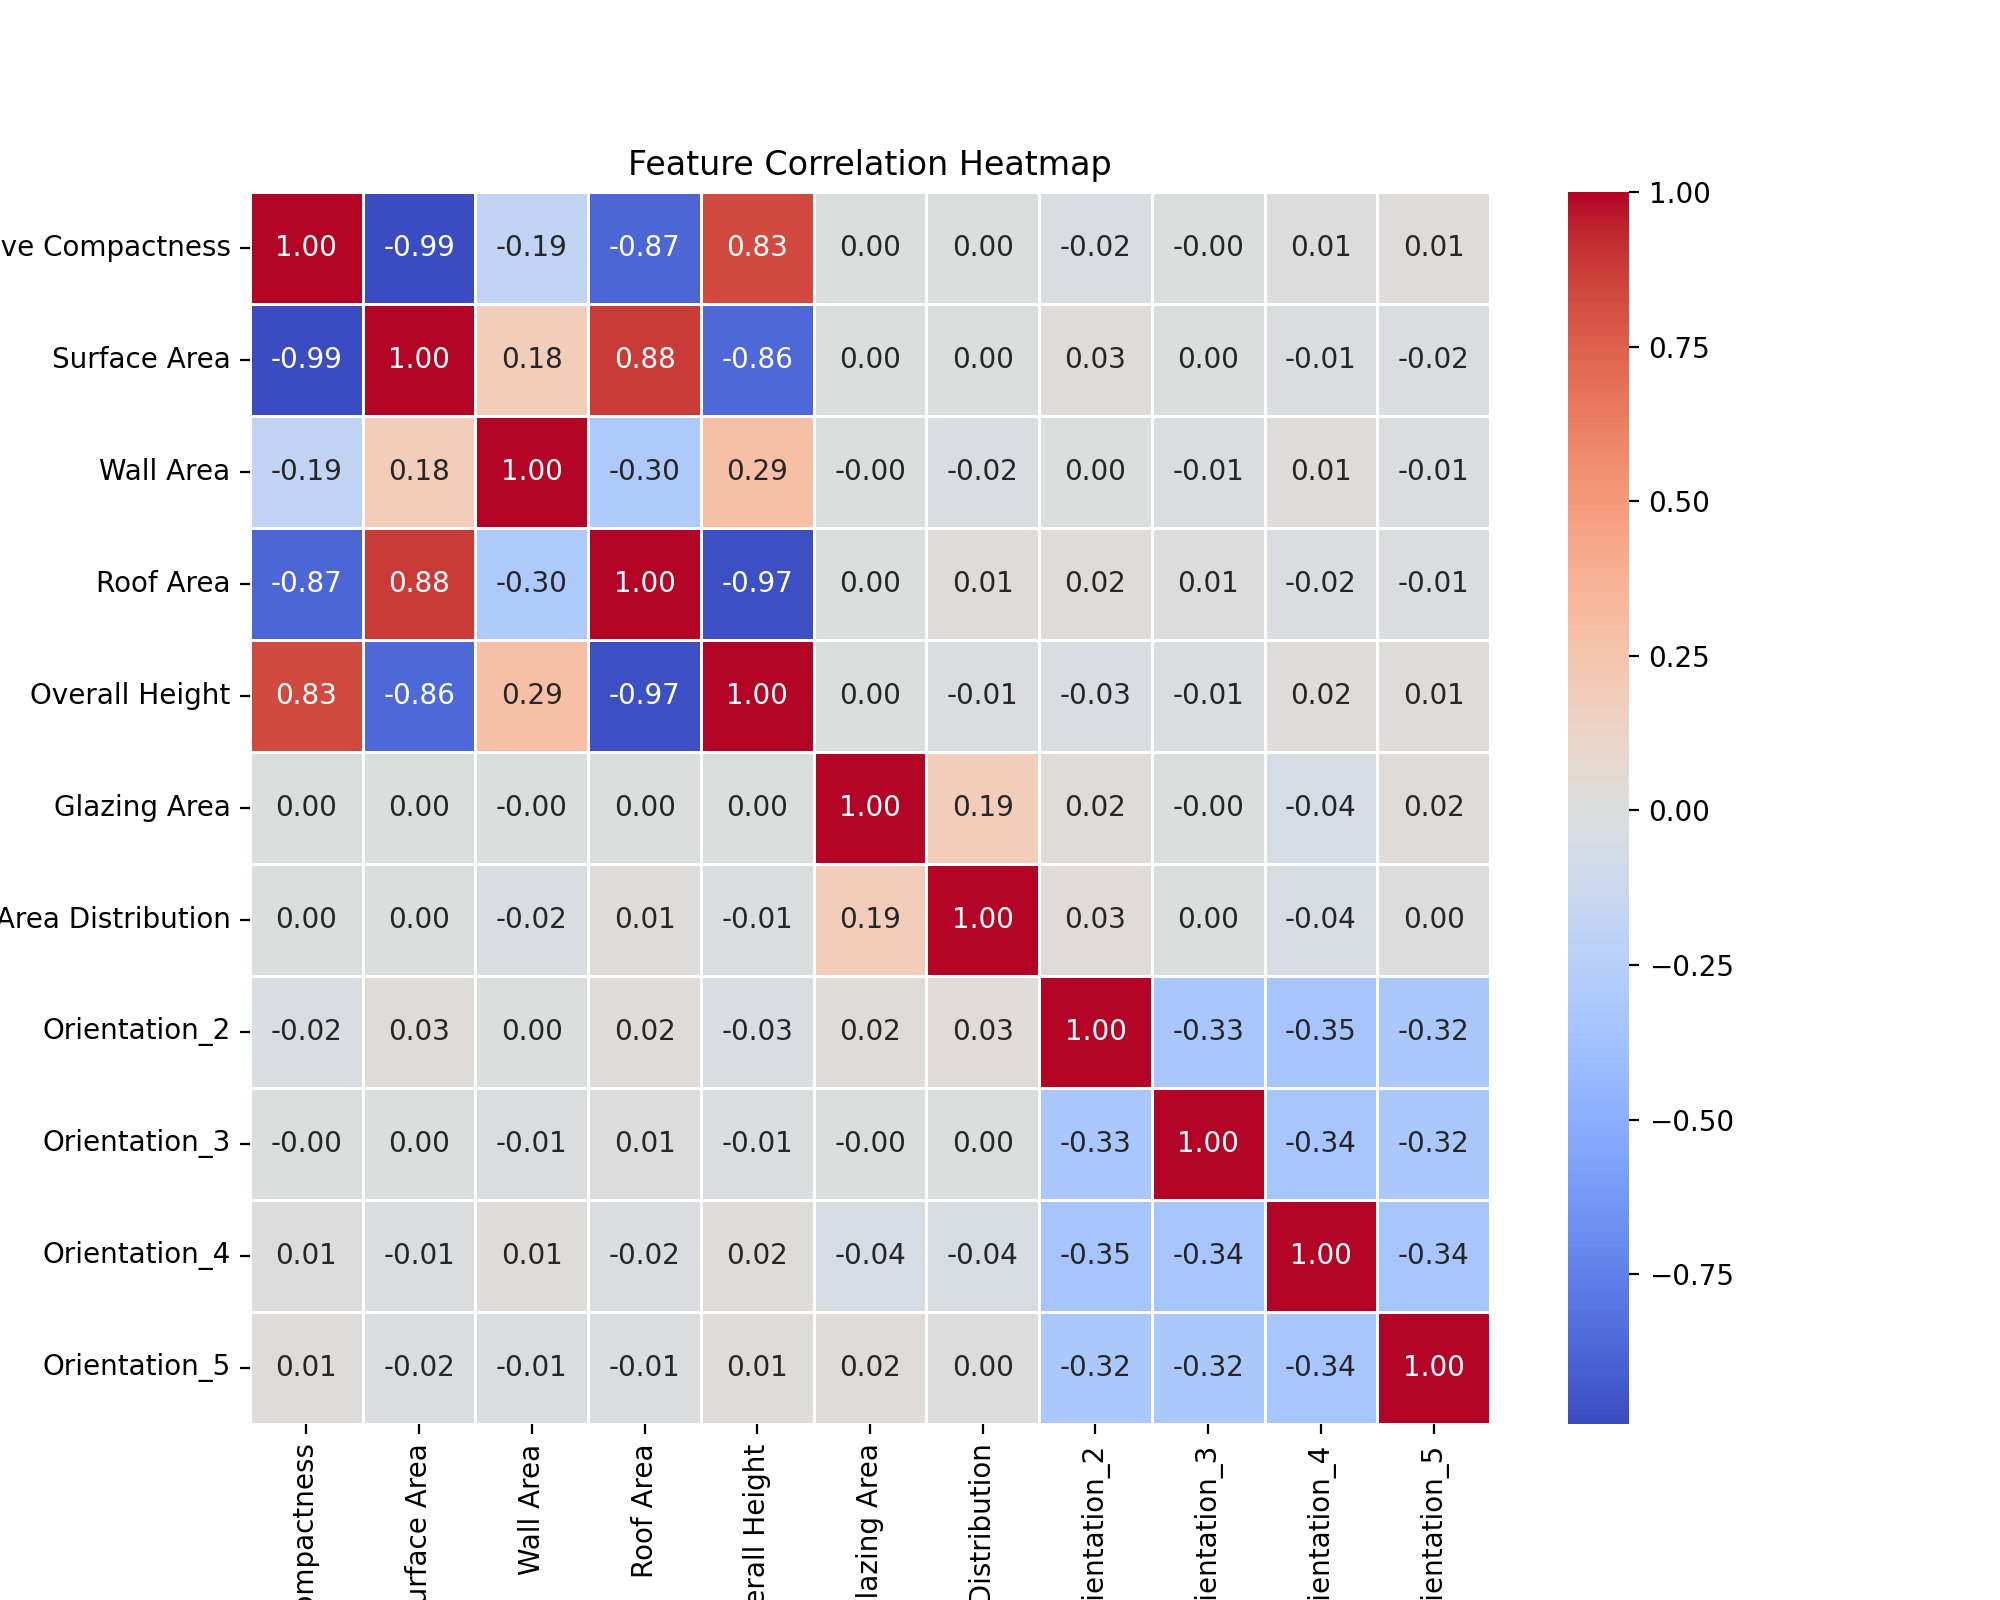
\includegraphics[width=.7\linewidth]{Feature_Correlation_Heatmap.png}
    \caption{Feature Correlation Heatmap}
    \vspace{-1em} % Reduce vertical spacing
\end{figure}

\subsection{Outlier data distribution exploration}
No significant observations to take actions.

\begin{figure}[H]  
    \centering
    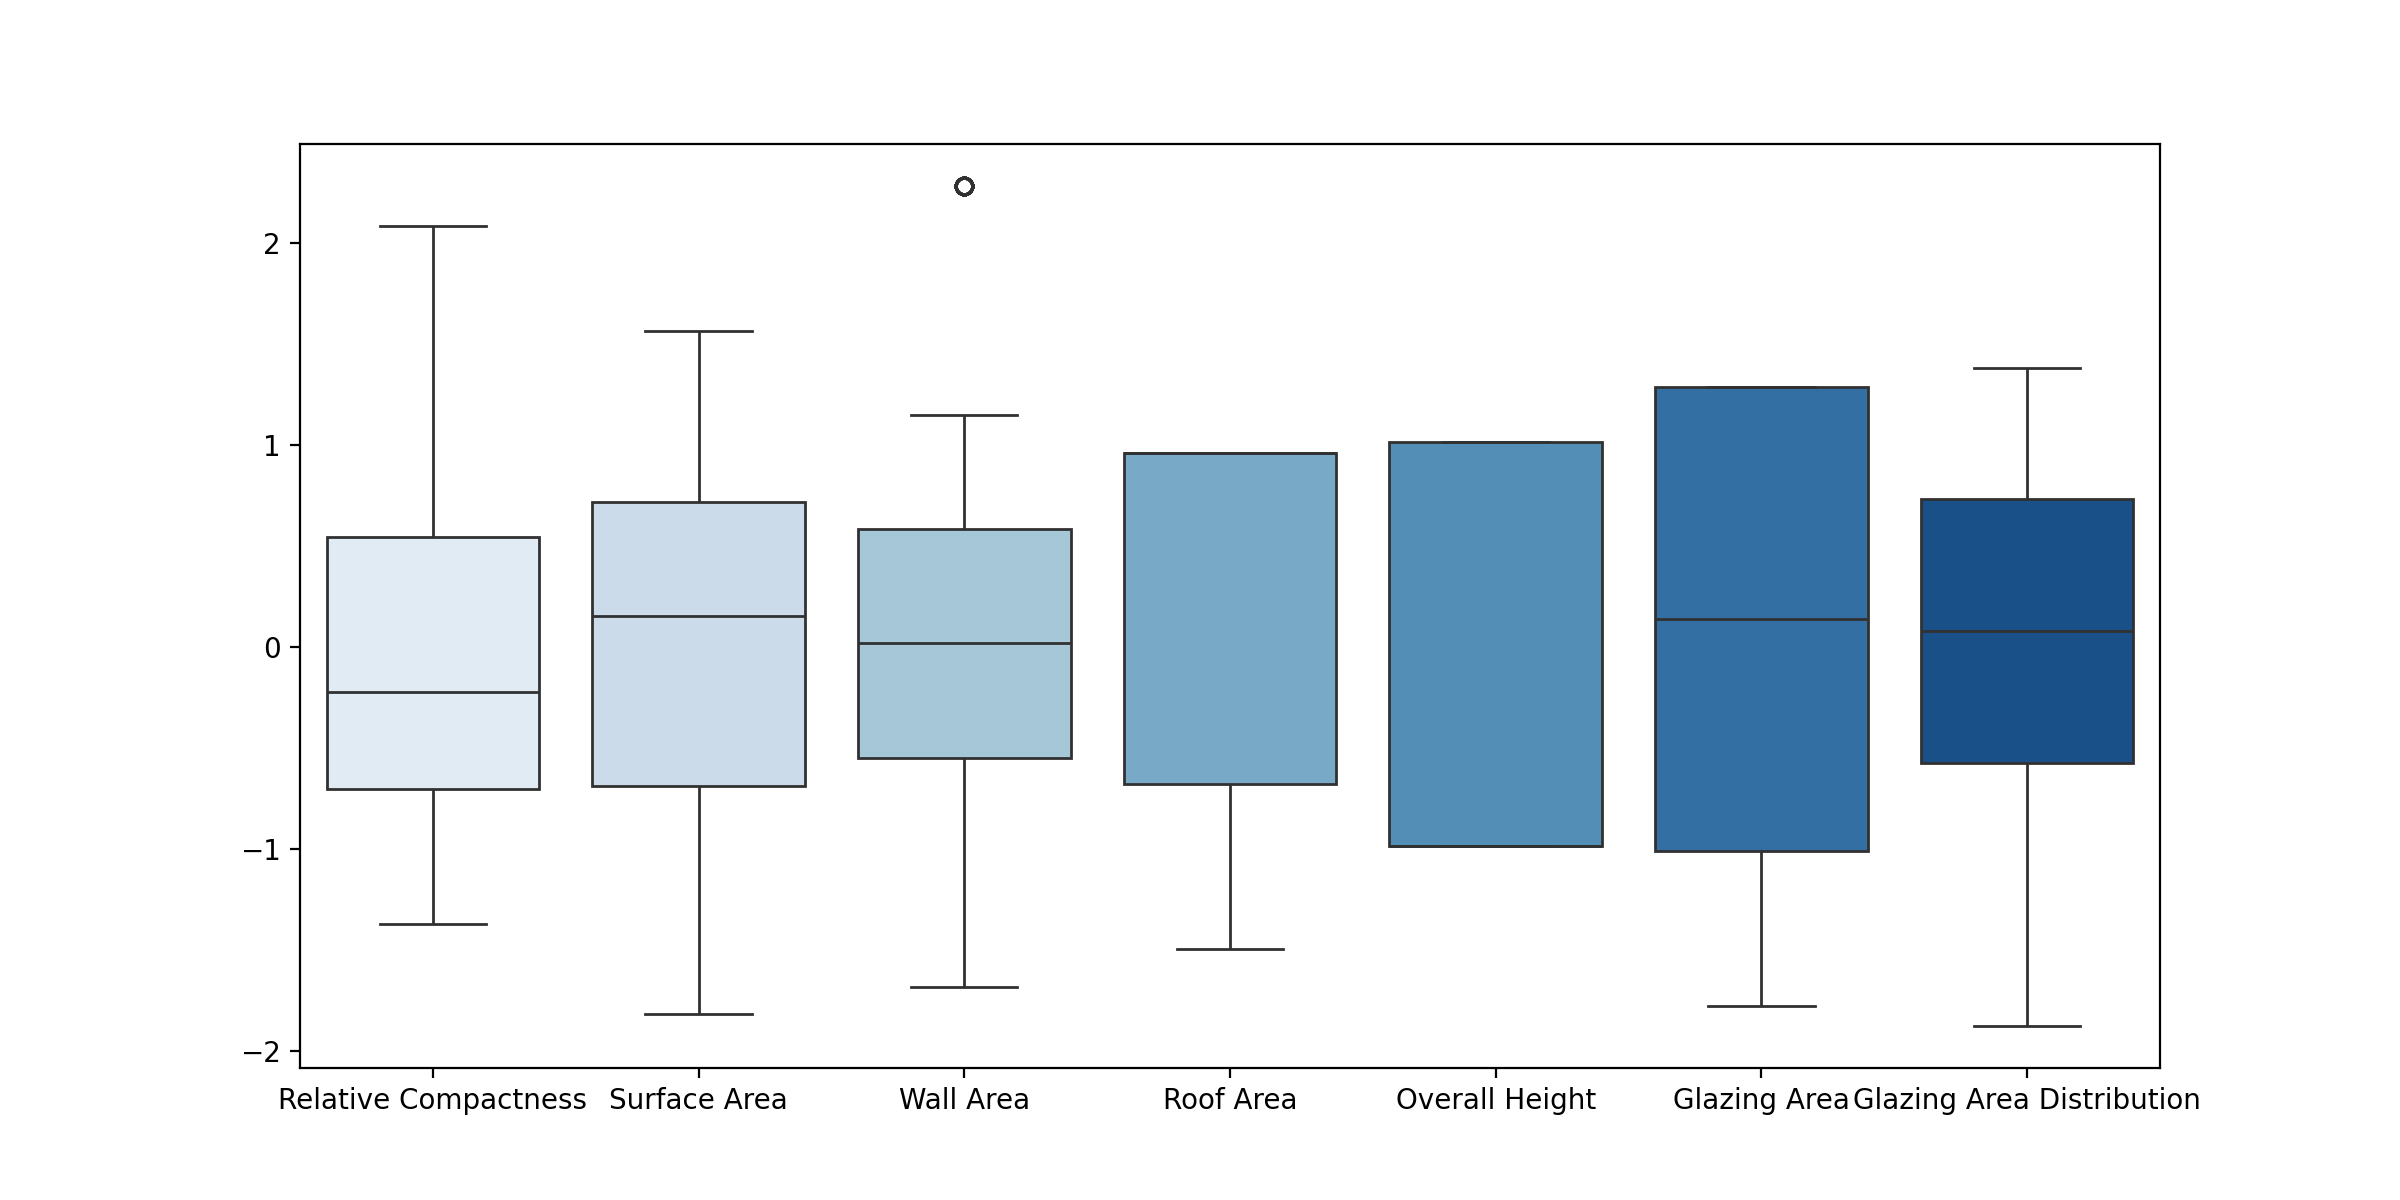
\includegraphics[width=1\linewidth]{BoxPlot.png}
    \caption{Feature Correlation Heatmap}
    \vspace{-1em} % Reduce vertical spacing
\end{figure}
\subsection{Features Correlation Matrix}

\section{Methodology}
In this study, we performed hyperparameter tuning using Grid Search, testing multiple machine learning algorithms to identify the best-performing model. The following algorithms were evaluated:

\subsection{Metrics Used}

\subsection*{Root Mean Squared Error (RMSE)}

The RMSE measures the square root of the average squared differences between predicted and actual values. It is given by:

\[
\text{RMSE} = \sqrt{\frac{1}{n} \sum_{i=1}^n (y_i - \hat{y}_i)^2}
\]

Where:
\begin{itemize}
    \item \( y_i \): Actual value,
    \item \( \hat{y}_i \): Predicted value,
    \item \( n \): Number of samples.
\end{itemize}

\subsection*{R-Squared (R²)}

The R-Squared score measures the proportion of variance explained by the model. It is defined as:

\[
R^2 = 1 - \frac{\sum_{i=1}^n (y_i - \hat{y}_i)^2}{\sum_{i=1}^n (y_i - \bar{y})^2}
\]

Where:
\begin{itemize}
    \item \( y_i \): Actual value,
    \item \( \hat{y}_i \): Predicted value,
    \item \( \bar{y} \): Mean of actual values,
    \item \( n \): Number of samples.
\end{itemize}

\subsection{Pre-processing Algorithms}

\begin{itemize}
    \item \textbf{Standard Feature Regularization:} Standardizes features by centering them at zero and scaling to unit variance:
    \[
    z = \frac{x - \mu}{\sigma}
    \]
    Where:
    \begin{itemize}
        \item \( x \): Original feature value.
        \item \( \mu \): Mean of the feature.
        \item \( \sigma \): Standard deviation of the feature.
    \end{itemize}

    \item \textbf{One-Hot Encoding (OHE):} Converts a categorical variable into binary features, one for each class:
    \[
    \text{OHE}(x) = [x_1, x_2, \dots, x_k], \quad x_i \in \{0, 1\}, \quad \sum_{i=1}^k x_i = 1
    \]
    Where:
    \begin{itemize}
        \item \( k \): Number of unique classes.
        \item \( x_i \): Binary variable indicating presence (\( 1 \)) or absence (\( 0 \)) of class \( i \).
    \end{itemize}

    \item \textbf{Principal Component Analysis (PCA):} PCA reduces dimensionality by transforming data into a new set of axes (principal components). The optimal number of components (axes) can be found iteratively using Grid Search with Cross-Validation (2-folds):
    \begin{itemize}
        \item Each fold evaluates the cross-validation score.
        \item Grid Search determines the number of principal components that maximize the model's performance.
    \end{itemize}
\end{itemize}

\subsection{Linear Regression Model}
If there aren't regularization techniques and the instance set is not too large, the solver will use the normal equation to compute weights, unless specified otherwise.

\subsection{Hyperparameter Tuning}
Grid search was used to determine the best number of axes in PCA. This is mainly for the sake of study, as no significant improvement is expected.

\begin{table}[h!]
    \centering
    \caption{Hyperparameter Combinations and Corresponding Test Scores with 2 K-folds}
    \label{tab:hyperparam_scores}
    \begin{tabular}{lcc}
    \toprule
    \textbf{Hyperparameter Combination} & \textbf{Mean Test Score} & \textbf{Rank Test Score} \\
    \midrule
    Preprocessing num pipeline PCA components = 5 & 0.8945 & 1 \\
    Preprocessing num pipeline PCA components = 3 & 0.8384 & 2 \\
    Preprocessing num pipeline PCA components = 1 & 0.6438 & 3 \\
    \bottomrule
    \end{tabular}
\end{table}

\section{Results and Discussion}

The results are promising. The model performs reasonably well with a 95 percent variance acceptance.

\subsection{Model Benchmark}

\begin{table}[h!]
    \centering
    \caption{Training and Test Set Performance Metrics}
    \label{tab:performance_metrics}
    \renewcommand{\arraystretch}{1.2} % Adjust row spacing
    \begin{tabular}{lcc}
        \toprule
        \textbf{Metric} & \textbf{Training Set} & \textbf{Test Set} \\
        \midrule
        RMSE            & 3.0672               & 3.1580           \\
        \( R^2 \)       & 0.9481               & 0.9506           \\
        \bottomrule
    \end{tabular}
\end{table}

\subsection{Feature Relevance to Determine Heating Efficiency}

The most important PCA component is: PC2.
The most important feature is: Wall Area.
 The worst feature is: Relative Compactness.

\begin{figure}[H]  
    \centering
    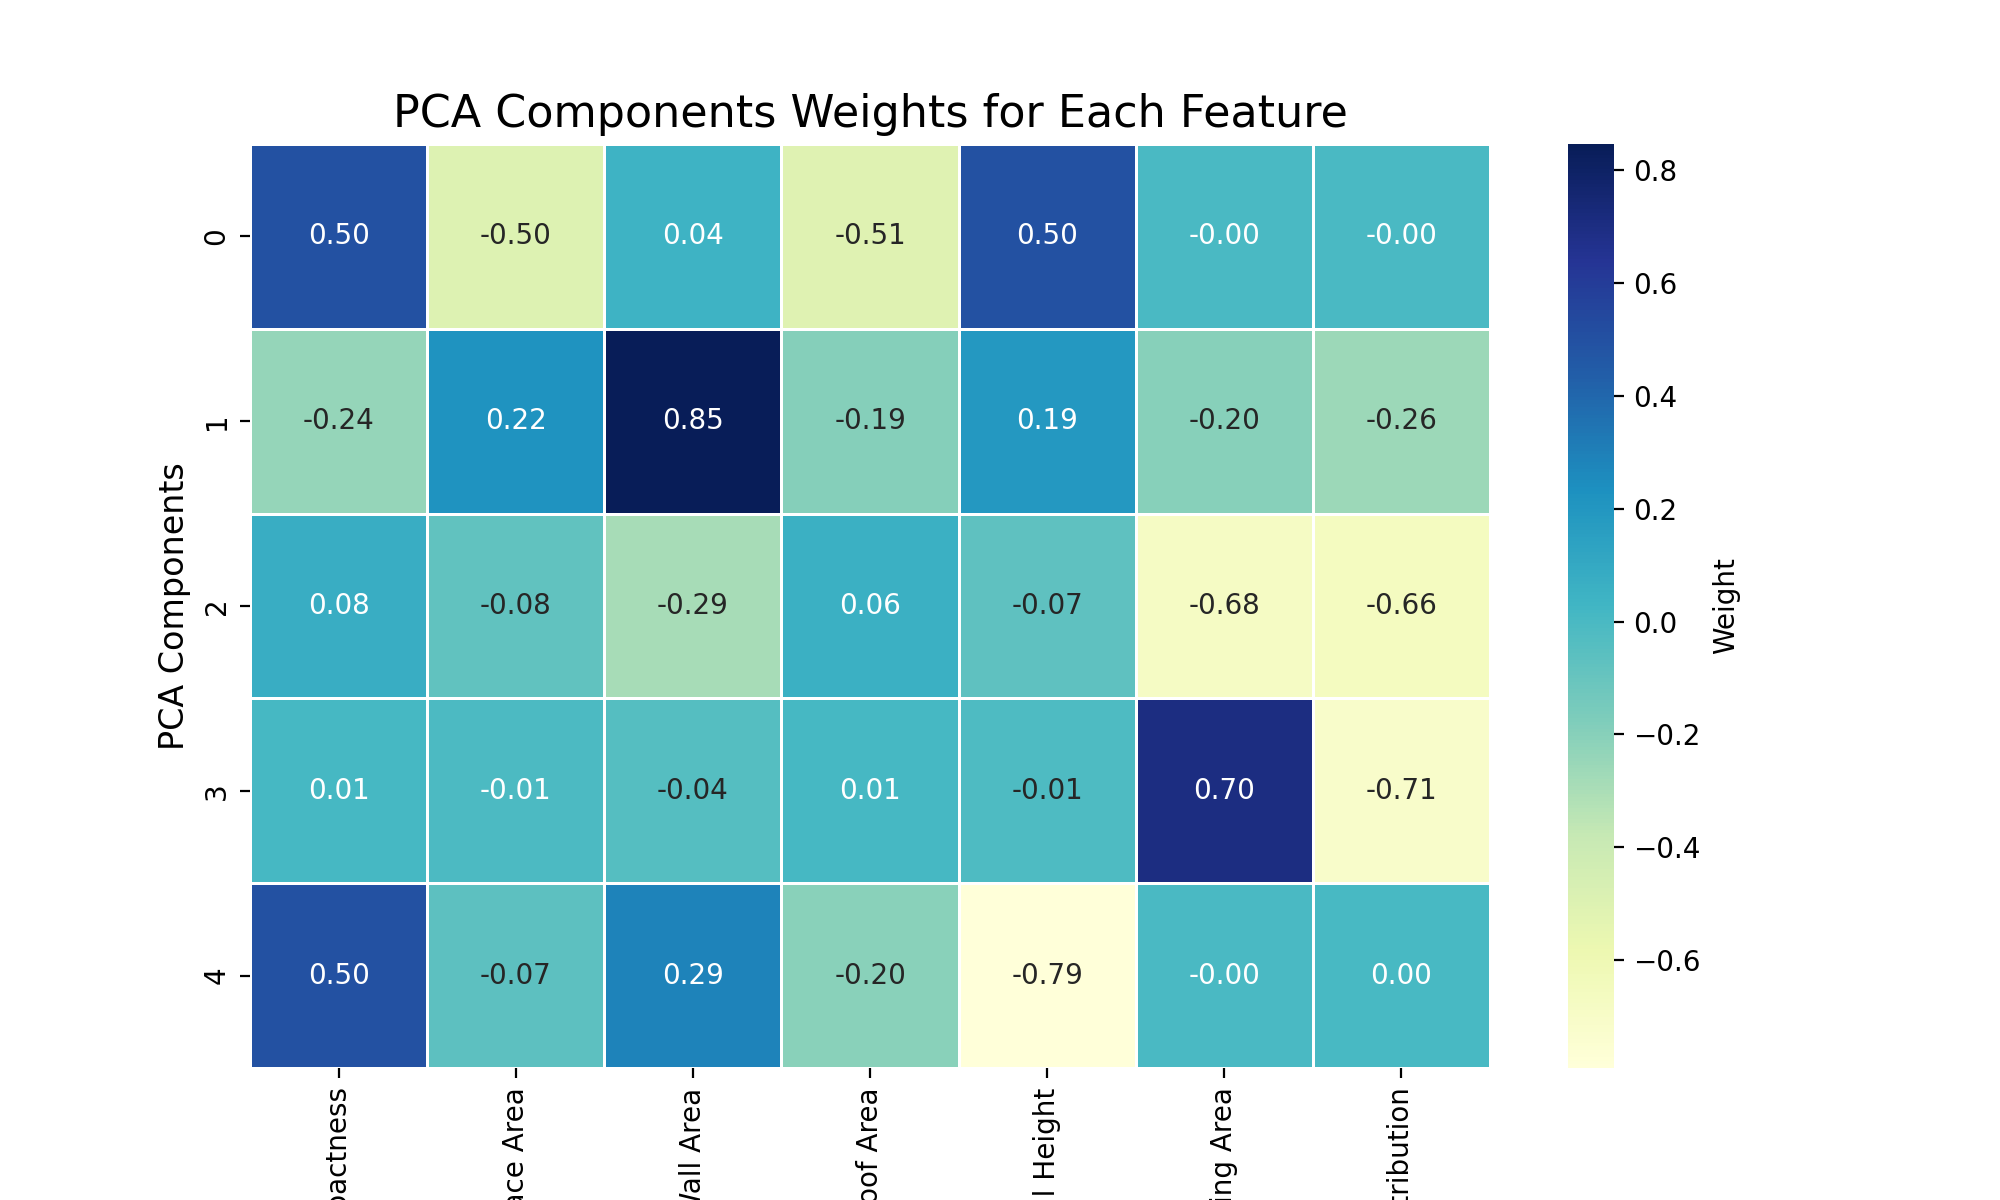
\includegraphics[width=1\linewidth]{PCAComponents.png}
    \caption{Features Correlation Heatmap}
    \vspace{-1em} % Reduce vertical spacing
\end{figure}

The wall area is the strongest feature, which is something that it does make sense which official data
for heating load, as surface increases so the heat exchange surface. It is on the eyes of the study a reasonable 
conclusion.

 However, the principal components themselves don’t provide a clear interpretation of the properties along each axis. If additional features were included in the analysis, I would expect the new axes to become more closely correlated with the wall area feature.

\section{Conclusion and Further Analysis}

The regression model effectively explains both cooling and heating efficiency, demonstrating a strong correlation with the non-synthetic dataset. Although the model is relatively simple, it shows promising results. However, several improvements can be made:

- We analyzed an averaged result between cooling load and heating load; however, it might be valuable to perform separate analyses for each target variable individually.
- There is a wealth of data available on building construction parameters. By scaling the model, we could incorporate additional features such as geographic location, building materials, and city-specific heat signatures.

\appendix
\section{Jupyter notebook}
Code used for this analysis \cite{arath2024github}.

\label{sec:appendix}
\bibliographystyle{alpha}
\bibliography{bli}

\end{document}
